\section{計算領域(格子数・解像度・MPIプロセス数)の指定}
\label{sec:domain}
%=======================================================================

水平格子間隔と格子数が計算領域を決定するのは言うまでもないが、
SCALEではMPIプロセス数も考慮する必要がある。
図X\textcolor{red}{追加予定}%\ref{fig:domain}
は、計算領域、及び、水平格子間隔、格子数、MPIプロセス数の関係を示している。


%\begin{figure}[h]
%\begin{center}
%  \includegraphics[width=0.9\hsize]{./figure/scale_grid.png}\\
%  \caption{SCALE-RMモデルの実行過程}
%  \label{fig:scale_grid}
%\end{center}
%\end{figure}


計算領域は、MPIプロセス数(n=\verb|PRC_NUM_X|$\times$\verb|PRC_NUM_Y|)が
2以上の時は、計算領域を水平方向にn個に分割して行う。
namelistで設定する格子数(\verb|IMAX|, \verb|JMAX|, \verb|KMAX|)は、
1つのMPIプロセスが担当する格子点数を与える仕様となっている。
以上の関係から、計算領域全体の総格子点数は、
\begin{eqnarray}
 総格子数 = (\verb|IMAX| \times \verb|PRC_NUM_X|)
   \times (\verb|JMAX| \times \verb|PRC_NUM_Y|)
   \times (\verb|KMAX| )  \nonumber
\end{eqnarray}
である。次節以降では、MPIプロセス数、格子数、格子間隔、それぞれの設定方法について詳しく説明する。


\subsection{MPIプロセス数}

MPIプロセス数は、各confファイルの\verb|PARAM_PRC|で指定する。
先に述べた通り、SCALEの入出力ファイルは、MPIプロセス毎に分割されている。
そのため、MPIプロセス数を変更すると分割ファイル数も必ず変わることになる。
従って、例えば、2-MPI並列用に作成した初期値ファイルは、
4-MPI並列のモデル実行には使用できない。
MPIプロセス数を変更するには、
\verb|pp_***.conf|、\verb|init_***.conf|、\verb|run_***.conf| の
すべてを編集・変更し、\verb|pp|, \verb|init| から行う必要がある。\\

\noindent {\small {\gt
\ovalbox{
\begin{tabularx}{140mm}{lX}
\verb|&PARAM_PRC| & \\
\verb| PRC_NUM_X       = 2,| & ; X方向(東西方向)のMPI並列分割数 \\
\verb| PRC_NUM_Y       = 1,| & ; Y方向(南北方向)のMPI並列分割数 \\
\verb|/|\\
\end{tabularx}
}}}\\


全MPIプロセス数は、\verb|PRC_NUM_X| $\times$ \verb|PRC_NUM_Y|  となり、
上記の例では、X方向に2分割、Y方向に1分割(分割なし)の
2-MPI並列ということになる。

実行時にMPIコマンドに指定するMPIプロセス数は、
この総MPIプロセス数を指定しなければならない。
この条件を満たさない場合は、下記のメッセージが
LOGファイルなどに出力されて計算は異常終了する。

\noindent {\small {\gt
\ovalbox{
\begin{tabularx}{140mm}{l}
\verb|xxx total number of node does not match that requested. Check!| \\
\end{tabularx}
}}}\\



\subsection{水平・鉛直格子数}
%-----------------------------------------------------------------------

格子数の設定は、configureファイルの\verb|PARAM_INDEX|で行う。
以下で設定する水平格子数の値は、
1つのMPIプロセス当たりの値であることに注意が必要である。\\

\noindent {\small {\gt
\ovalbox{
\begin{tabularx}{140mm}{lX}
\verb|&PARAM_INDEX| & \\
\verb| KMAX = 97,|  & 鉛直層数 \\
\verb| IMAX = 20,|  & X方向の格子点数 \\
\verb| JMAX = 2, |  & Y方向の格子点数 \\
\verb|/|\\
\end{tabularx}
}}}\\



\subsection{水平・鉛直格子間隔}
\label{sec:gridinterv}
%-----------------------------------------------------------------------
SCALEでは、格子点の位置を均等間隔に設定することも、
任意の格子点位置を直接指定することもできる。
以下で説明する
\textcolor{red}{\bf 格子間隔の設定は、pp\_***.conf、init\_***.conf、run\_***.confの
configファイルの間で一致させなければならないことに注意が必要である。}
また、以下で設定する値は、MPIプロセス当たりの値であることに注意が必要である。


\subsubsection{等間隔で設定する場合}
%-----------------------------------------------------------------------&
configファイルの\verb|PARAM_GRID|の\verb|DX|、\verb|DY|、\verb|DZ|に
それぞれ、東西、南北、鉛直方向の格子間隔を指定する。
水平格子間隔は等間隔\footnote{緩和領域は除く(第\ref{sec:buffer}節参照)}でしか設定できない。\\

\noindent {\small {\gt
\ovalbox{
\begin{tabularx}{140mm}{lX}
\verb|&PARAM_GRID  | & \\
\verb| DX = 500.D0,| & ; X方向(東西方向)の格子間隔\\
\verb| DY = 500.D0,| & ; Y方向(南北方向)の格子間隔\\
\verb| DZ = 500.D0,| & ; Z方向(鉛直方向)の格子間隔\\
\verb|/|\\
\end{tabularx}
}}}\\


\subsubsection{任意の格子点位置を指定}
%-----------------------------------------------------------------------&
この設定方法は、鉛直方向にのみ有効である。
SCALEの格子系はArakawa-Cグリッド、
およびLorenzグリッドであるため、水平方向と鉛直方向ともに
スタッガード点(1/2ずれた点)に変数が定義されている。
コントロールボリュームに対して中心点に位置する格子点を
Center Pointと呼び、コントロールボリュームの面に位置する格子点
(Center Pointに対して1/2ずれている)をFace Pointと呼ぶ。
SCALEでは、これらの頭文字と方向を組み合わせて
\verb|CX、CY、CZ|や\verb|FX、FY、FZ|と定義している。
(図\ref{fig:scale_grid})。


\begin{figure}[h]
\begin{center}
  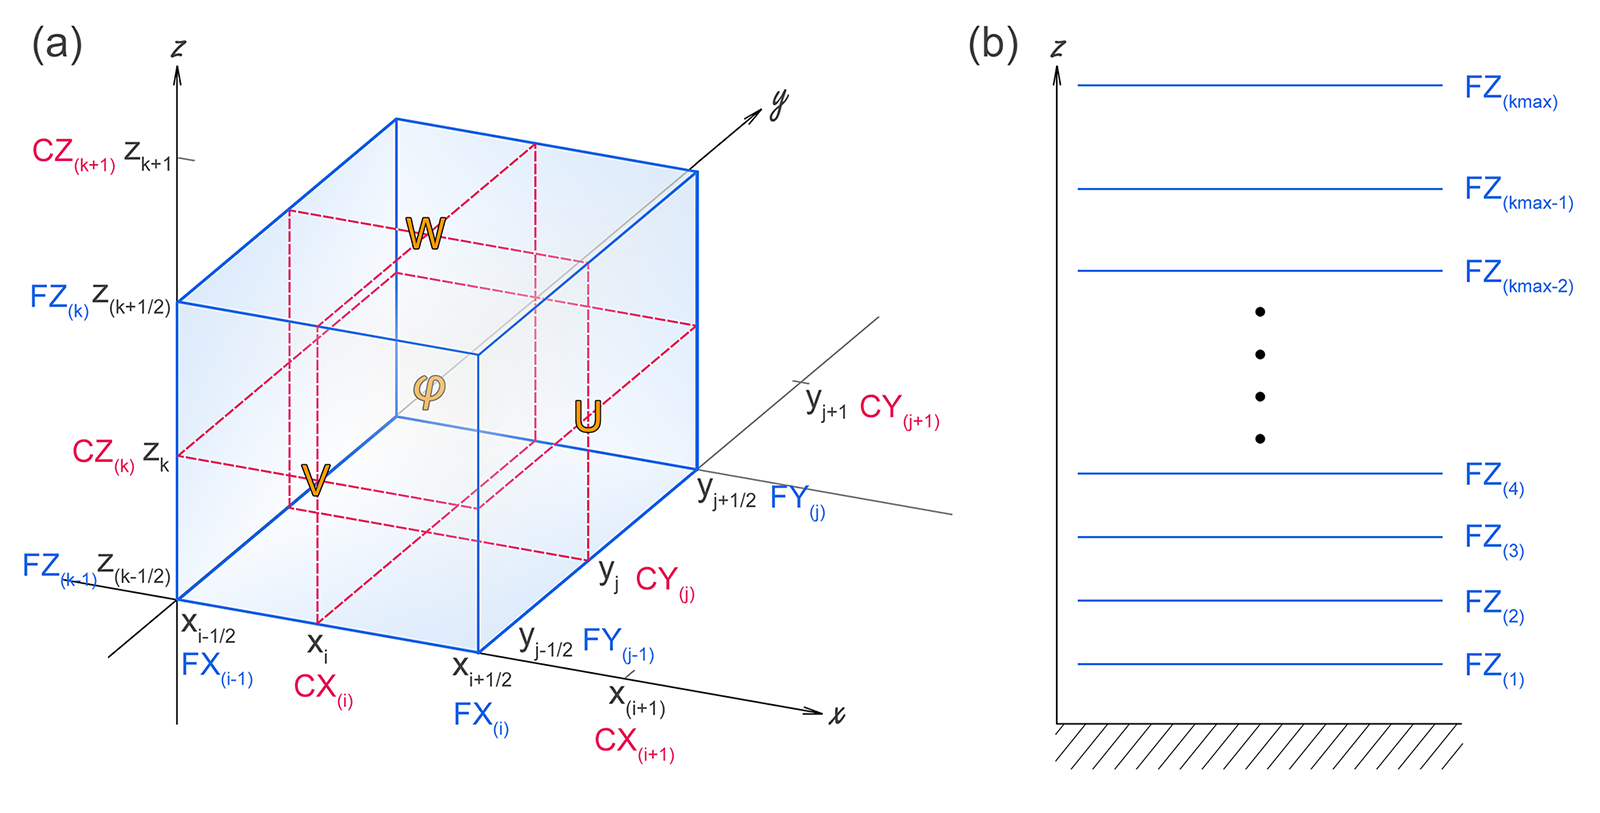
\includegraphics[width=0.8\hsize]{./figure/Center-Face.eps}\\
  \caption{SCALE-RMの格子の定義}
  \label{fig:scale_grid}
\end{center}
\end{figure}

直接格子点の位置を指定する場合は、Z方向のFace Pointの位置を
\verb|FZ(:)|に指定
\footnote{指定の際には、シミュレーションの計算精度
(モデルのコンパイル時に指定した浮動小数点の精度。デフォルトでは倍精度)を用いることが望ましい。}
(単位はメートル[m]) すれば良い。
\verb|FZ(:)|で指定する値の数は、鉛直層数(\verb|PARAM_INDEX|の\verb|KMAX|)と一致させる必要がある。
例として理想実験のチュートリアルのrun.confファイル
(run\_R20kmDX500m.conf)を下記に示す。\\

\noindent {\small {\gt
\ovalbox{
\begin{tabularx}{140mm}{lX}
\verb|&PARAM_GRID|     & \\
\verb| DX = 500.D0,|   & X方向の格子間隔(等間隔)\\
\verb| DY = 500.D0,|   & Y方向の格子間隔(等間隔)\\
\verb| FZ(:) = |       & Z方向のFace pointの位置[m] \\
\verb|    80.000000000000000      ,| & \\
\verb|    168.00000190734863      ,| & \\
\verb|    264.80000610351567      ,| & \\
\verb|     〜 中略 〜|           & \\
\verb|    14910.428862936289      ,| & \\
\verb|    15517.262523292475      ,| & \\
\verb|    16215.121232702089      ,| & \\
\verb|    17017.658748523147      ,| & \\
\verb|    17940.576891717363      ,| & \\
\verb|    19001.932756390710      ,| & \\
\verb|    20222.492000765058      ,| & \\
\verb| BUFFER_DZ = 5000.D0,|          & 第\ref{sec:buffer}節参照\\
\verb| BUFFFACT  =   1.0D0,|          & 第\ref{sec:buffer}節参照\\
\verb|/|\\
\end{tabularx}
}}}\\


格子点位置を任意に設定できるといっても、設定が悪いと計算不安定につながる。
鉛直層設定の作成をサポートするツールを
\verb|scale/scale-rm/util/makevgrid/|
\footnote{``make\_vgrid.f90''というFortranプログラムと
いくつかのサンプルnamelistが用意されている。}
使って生成することを勧める。
ツールをコンパイルして実行すれば直ちにconfigファイルに貼り付けて使用できる
\verb|FZ|の設定が作成される。
